\section{Υλοποίηση στον Καθρέφτη}
\label{sec:os_mirror}
Στην παράγραφο αυτή φαίνεται η μεταφορά των παραπάνω υλοποιήσεων στον πραγματικό καθρέφτη. Η κατασκευή του καθρέφτη πραγματοποιήθηκε στην διπλωματική της Κωνσταντίνας Λέλοβα \cite{nantia_mirror}. Στο Σχήμα \ref{fig:front_page} απεικονίζεται η βασική οθόνη του λειτουργικού συστήματος. Η επιφάνεια του καθρέφτη είναι ανακλαστική προκειμένου να φαίνεται το είδωλο του εικονιζόμενου, ενώ επιτρέπεται και η απεικόνιση των Widgets από την οθόνη. Αριστερά πάνω φαίνεται το Widget του καιρού, δεξιά πάνω ένα ρολόι με το ημερολόγιο και στη μέση ένα τυχαίο μήνυμα καλωσόρισης για τον χρήστη. Τέλος, κάτω δεξιά υπάρχει ένα διακριτικό κείμενο που γράφει "listening..." το οποίο βοηθάει τον χρήστη να καταλάβει πότε ο καθρέφτης ακούει για εντολές.

\begin{figure}[h]
	\centering
	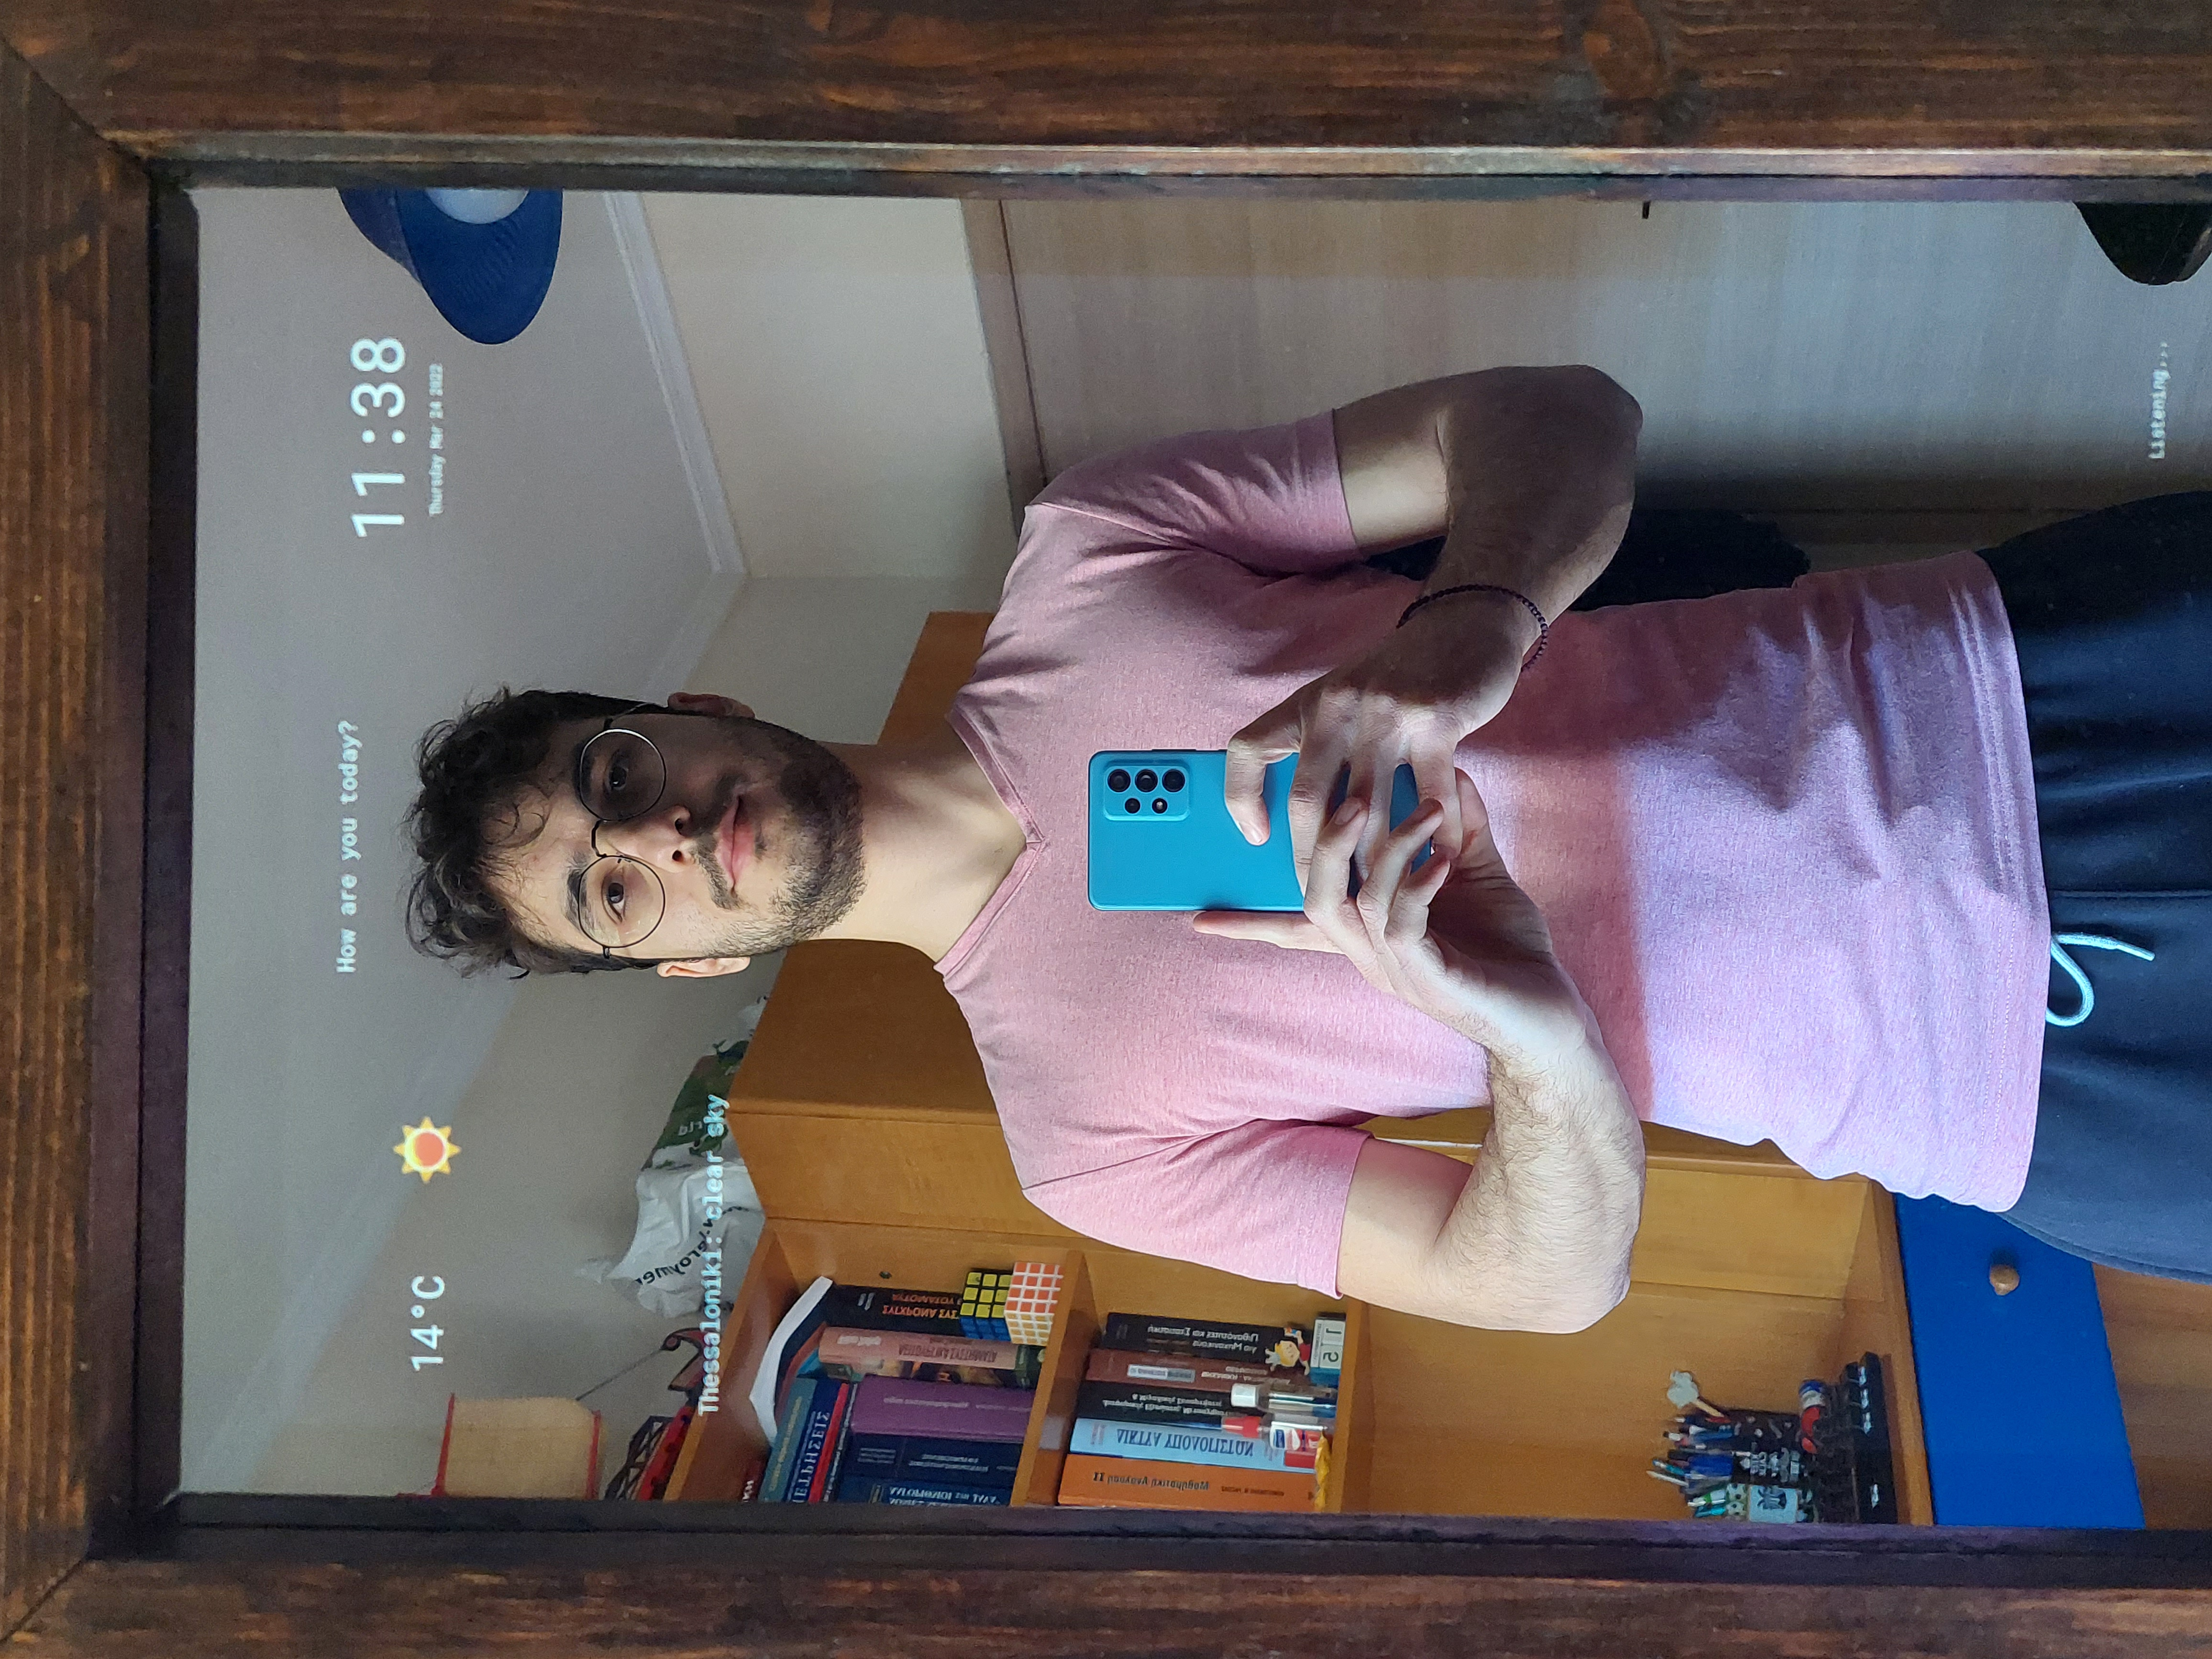
\includegraphics[scale=0.08,angle=270]{images/chapter4/front_page.jpg}
	\caption{Μεταφορά την αρχικής σελίδας του λειτουργικού στον φυσικό καθρέφτη}
	\label{fig:front_page}
\end{figure}